\documentclass[../main-v1.tex]{subfiles}
\begin{document}
\chapter{Data Placement \hideme{draft 3/10 moved from end to right after data placement } }
\label{ch:place}
\todo{Stu Fuess requests text on tape}
%%%%%%%%%%%%%%%%%%%%%%%%%%%%%%%%
%\section{xyz}
%\label{sec:places:xyz}  %% fix label according to section

\section{Current Status}

DUNE relies on a multi-level data placement strategy that has grown out of the Fermilab fixed target program with elements from CERN fixed target experiments.  Figure \ref{fig:storage} illustrates the storage available to users. Reference \cite{bib:storage} provides a more detailed description. 

\subsection{Storage systems at Fermilab}

There are two general use cases considered for storage systems at Fermilab: production operations and analysis end users. Production operations is in general focused on utilization of large-scale storage elements. Analysis end users though utilize a wide variety of storage systems and typically log into on of a set of \dwords{vm}  which have disk mounts of varying size and level of backup. 

\begin{description}

    \item{\bf Local disk -}  There are small   volumes on local physical disks, directly
mounted on the machine hosting the \dword{vm} with direct links to the /dev/ location
used as temporary storage for infrastructure services (e.g. /var, /tmp).
These areas should be used to store certificates and tickets. These secure items are saved to local disk automatically with owner-read permission and other permissions disabled.
These local areas are usually very small and should not be used to store data files or for code development.
    
    \item{\bf Network Attached Storage}
    
     Users have access to POSIX compliant network attached storage areas with varying sizes and levels of backup. Network attached disks are not safe for storage of certificates and tickets.

 \begin{itemize} 
   \item Users are provided with a network mounted home area {\tt /nashome/} (usually 2 GB).    A valid Kerberos ticket is needed   to access files in the home area. Periodic snapshots are taken and available in "{\tt  /nashome/.snapshot}". There are additional network mounted areas for code development and small data analysis samples. 
\item {\tt /dune/app} is intended for code development and is  limited to 100 GB/user.  /dune/app has periodic snapshots in /dune/app/.snapshot

\item  {\tt /dune/data} and {\tt /dune/data2} are larger areas for fast analysis and code testing.  They are not backed up.  
\end{itemize}
 
The \dword{nas} disks {\tt /dune/app} and {\tt /dune/data} are not accessible as an output location from grid worker nodes. 
 
\item{\bf dCache -} Several PB of \dword{dcache}\cite{Millar:2014cfa} storage is available at several scales. \dword{dcache} storage is not fully POSIX compliant but \dword{nfs} mounts with limited functionality are available on Fermilab interactive machines. The \dword{dcache} storage is readable and writable from grid machines via \dword{xrootd} and transfer mechanisms such as \dword{ifdh}. It is expected that this is the main storage element for the output of both production and analysis distributed computing jobs.

\begin{itemize}
    \item {\tt /pnfs/dune/scratch}  is a scratch area used mainly for files returning from grid jobs.  Files are automatically removed to accommodate new files. Typical lifetimes are 1 month. 
     \item {\tt /pnfs/dune/persistent} is a $\approx 800$ TB area for persistent storage of user files.  Files must be removed by their owner. Half of this volume is currently controlled with physics group based quotas, while the other half will soon be trainsitioned to quota-controlled usage.
      \item {\tt /pnfs/dune/tape\_backed} is a $\sim 3.2$ PB disk cache sitting in front of the \dword{enstore} tape system. Files in this area are cataloged and tracked by the \dword{sam} system and, in future, by \dword{rucio}. Users may need to prestage samples to make them rapidly accessible. 
\end{itemize}

\item{\bf Tape -} DUNE shares the Public instance (separate from a CMS instance) of the tape storage infrastructure.  The physical system is currently (March 2022) composed of two IBM TS4500 tape libraries with LTO8 drives (72 total) with over 100 PB capacity per library.  In addition there is a legacy Oracle SL8500 library being replaced with a 150 PB capacity library (vendor selection and purchase pending).  Current DUNE utilization of the tape complex is 21 PB of the total (non-CMS) active utilization of 168 PB.
The tape storage software used is \dword{enstore}.  Fermilab is actively pursuing a transition to using the \dword{cern} \dword{cta} software, and plans a multi-year transition.


\item{\bf Distributed caching systems - } \dword{dune} makes use of the \dword{cvmfs} caching system to distribute code, flux and shower libraries and user grid executables. \dword{cvmfs} mounts are available on DUNE grid nodes. 



\begin{itemize}
    \item {\tt /cvmfs/ } mounts of DUNE-specific code,  shared executables such as \dword{larsoft}, and general utilities are distributed via \dword{cvmfs}. Version control is provided by the Fermilab \dword{ups} system. 
    
    \item \dword{stashcache} is used to deliver larger payloads such as flux files and shower libraries to grid jobs.
    
    \item A \dword{cvmfs}-based  {\tt dropbox} is also available to transfer user executables to grid jobs. 
    
    



\item{Collaboration disk stores}
DUNE collaborating institutions also contribute very substantial storage resources. These resources are populated and managed via \dword{rucio} and currently accessible via the \dword{sam} catalog. As with the Fermilab \dword{dcache} stores they are available via streaming and grid-copy mechanisms but are not mounted on interactive nodes. 
 \end{itemize}


\end{description}
\begin{dunefigure}
[Storage Schematic]
{fig:storage}
{Storage systems for DUNE computing.  Thick lines denote mounts while thinner lines denote transfer methods such as ifdc and xroot streaming.}
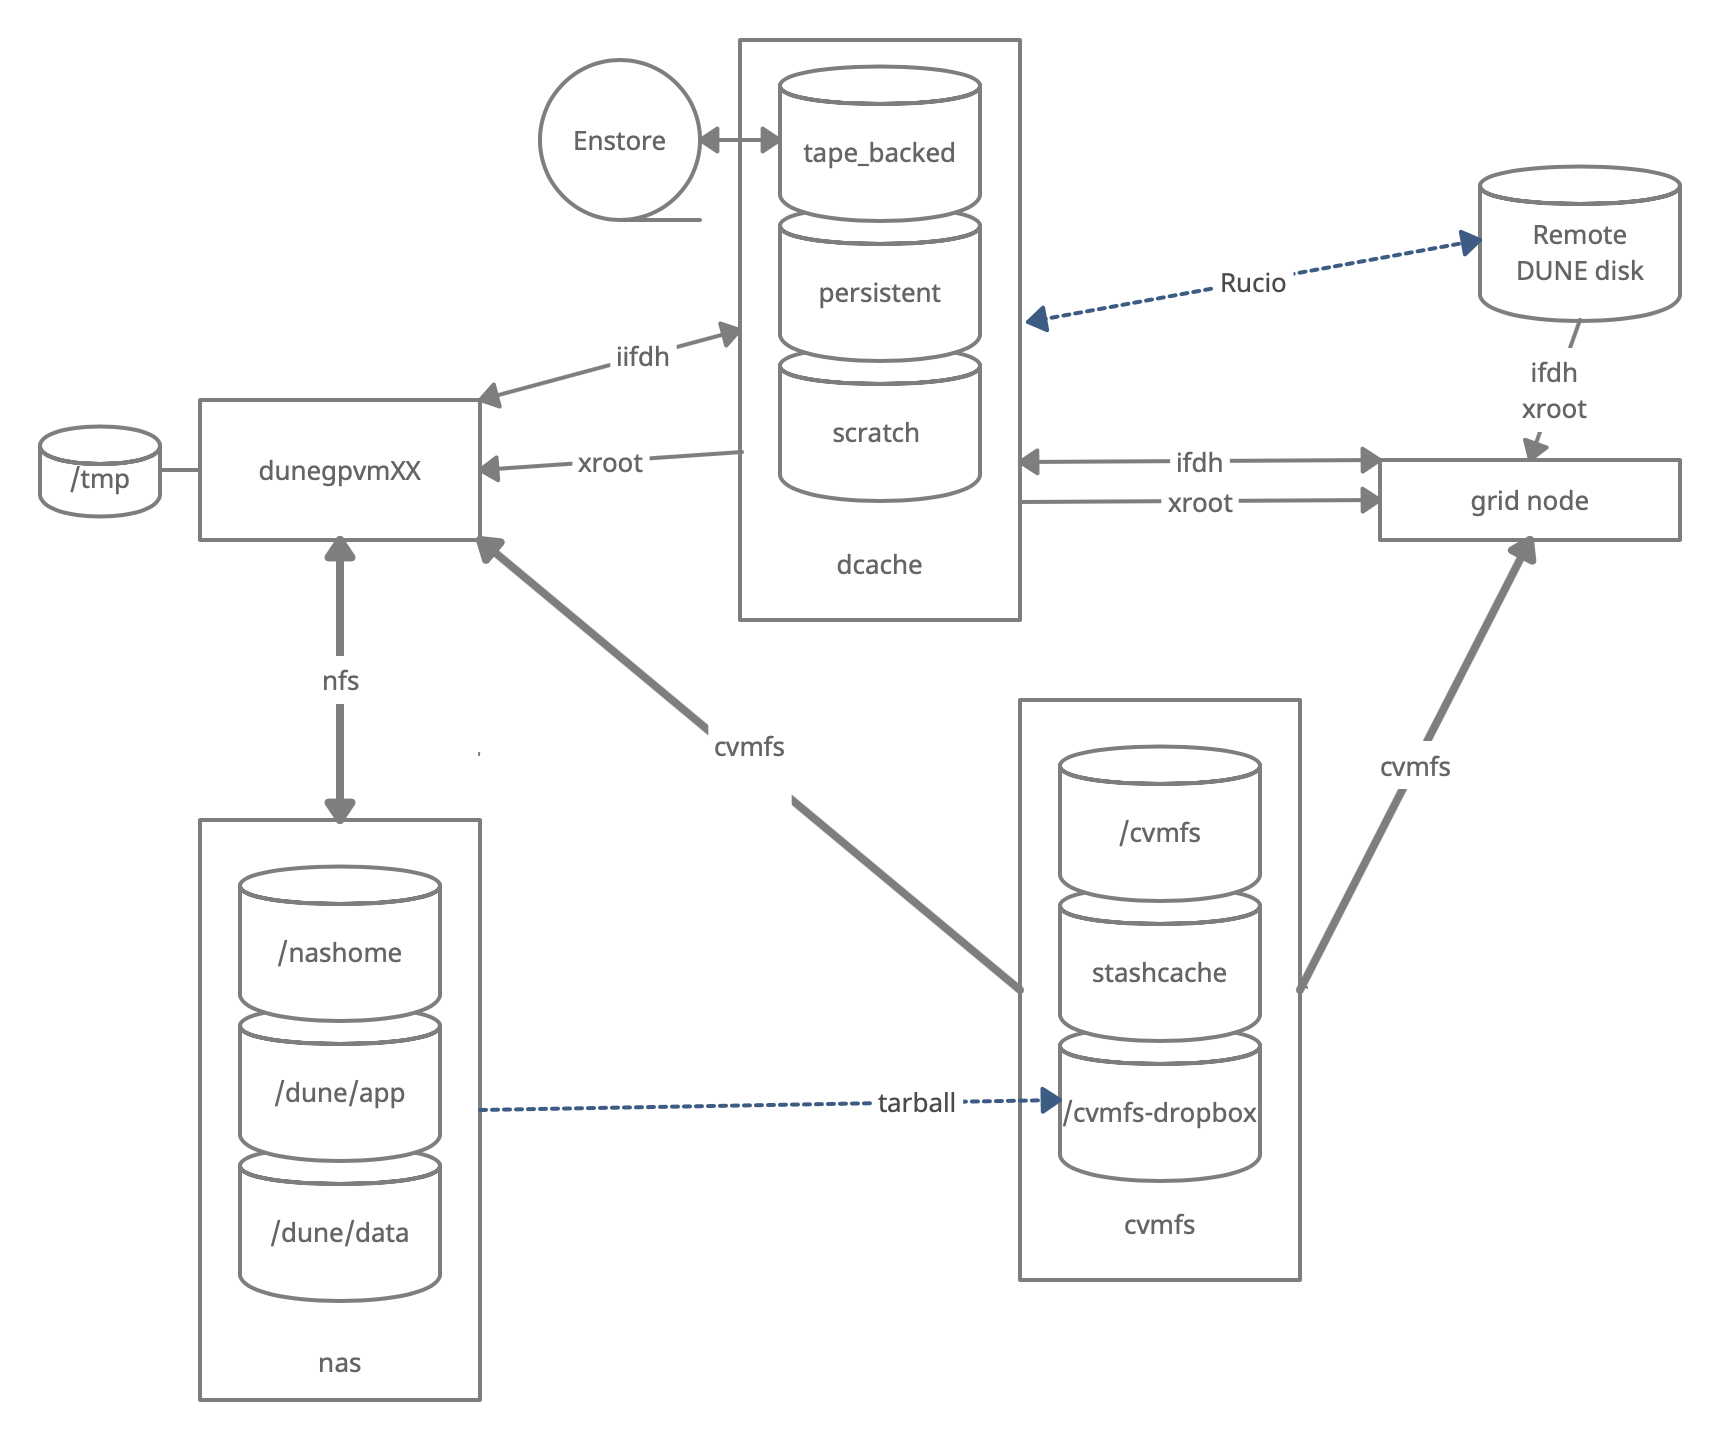
\includegraphics[width=0.8\textwidth]{graphics/DataManagement/StorageMap2.png}
\end{dunefigure}

\section{Storage systems at CERN}

Data at CERN are stored in the \dword{eos}, \dword{castor}, and \dword{cta} systems.  Some of this storage is under the control of the \dword{dune} \dword{rucio}
system, including a full copy of the \dword{protodune} raw data in \dword{castor}/\dword{cta}.  There is also substantial space for generic use by CERN-based users. The \dword{cvmfs} file systems are mounted at \dword{cern} and local users have access to the \dword{cern} batch resources through the normal \dword{dune} batch system which requires membership in the \dword{dune} \dword{vo} and through normal \dword{cern} submission systems.  

\section{Data Placement Strategy}

%Kirby this looks to me like it's done. \todo{What is our data placement policy and how is it implemented in the compute model. }

%\section{Data Placement Strategy}
%The following items describe the placement strategy that DUNE is utilizing to distributed the data globally:
%\begin{itemize}
%\item all \dword{dune} and \dword{pd} raw data to be located at two archival storage elements
%\item all production datasets to be stored on at least one archival storage element
%\item all production datasets will be actively located on at least two storage elements that are geographically separated by an ocean
%\item replication and distribution of raw data and production datasets will be implemented and performed by Rucio
%\item all datasets will have a well-defined data lifetime within the Rucio system
%\end{itemize}

\dword{dune} data has a large number of data access patterns based on the size, CPU/byte and frequency of access.   Major examples are:

\begin{description}
    \item{\bf Raw data -}  Raw data from the TPC detectors comes in 4-8 GB files which are generally run through reconstruction algorithms that take of order 5-10 sec/MB to process. Raw data is generally accessed a few times for calibration and reconstruction as part of an organized production effort.  
    \item{\bf Reconstructed data -}  Reconstructed data from \dword{pdsp} is around three times smaller  than the raw data once the raw TPC waveforms are dropped. It is accessed many times by end users for algorithm development, calibration and production of physics analysis samples.   Observed data access rates range from 1 to 40 MB/sec depending on the amount of reprocessing done to data. 
    \item{\bf Simulated data - } Simulated data are around twice as large as real data due to the large amount of simulation information that is kept.  Even after raw waveforms are dropped, records are still significantly larger. 
    \item{\bf Analysis samples - } End-user analysis samples are significantly smaller.  For example the 1 GeV ProtoDUNE simulation sample consists of $\sim$80,000 4 GB files while the reduced analysis sample is around 8 GB total.  
    \item{\bf Flux files - } Simulation and cross section extraction require access to large libraries of particle fluxes.  These are currently delivered via \dword{stashcache}. 
    
\end{description}

As described in the data volumes section \ref{ch:est}, raw data is kept in multiple tape copies but only kept on disk for the short period before calibration and reconstruction are complete.  If reprocessing is needed, the raw data must be prestaged to cache and work on optimizing this process is underway. Recent reconstructed data and simulation copies for users are kept on \dword{rucio}/\dword{sam} controlled disk, with one copy in the US and one in Europe if possible. Smaller final analysis samples are kept on user or group controlled persistent dcache or \dword{nas} areas. Rucio will perform replication and distribution of raw data and production datasets. 
 All datasets will have a well-defined data lifetime within the Rucio system. 
%\todo{Overlay policy - how does it work for MicroBooNE and NOvA}
\end{document}



